\section{Modos de Sincronización de Acciones utilizando Redes de Petri}
\label{sec:sincronizacion_cinta_transportadora}
En esta sección se analizan dos formas de llevar la sincronización de las
acciones mediante la utilización de las interfaces proporcionadas por el monitor
de Redes de Petri. Estos modos se denominan:
\begin{enumerate}
  \item Sincronización por aviso de ejecución.
  \item Sincronización por petición de ejecución.
\end{enumerate}

Para estudiar los modos de sincronización mencionados se hará uso de un caso de
ejemplo, descripto a continuación:

\begin{labeling}{description}
\item [Ejemplo]
Cinta transportadora con 3 estaciones. Se depositan piezas en la primer
estación de manera asincrónica. Cuando esto sucede, la cinta avanza a la
estación 1, donde un operario realiza una transformación a la pieza. Una vez el
operario realizó la transformación, presiona un pulsador y la cinta avanza a la
estación 2, donde el mismo operario empaqueta la pieza. El operario
presiona otro pulsador al finalizar su tarea y luego la cinta avanza una vez
más y la pieza se deposita en un contenedor. Una vez que la pieza llega al
contenedor se habilita el ingreso de una nueva pieza al proceso.
\end{labeling}

\begin{figure}[H]
    \centering
    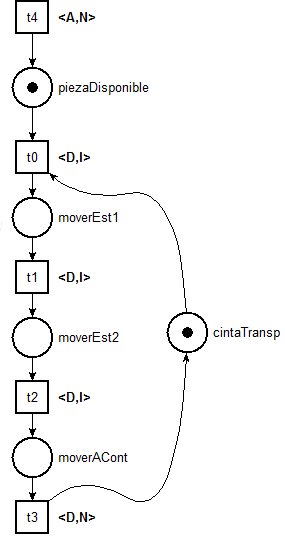
\includegraphics[height=100mm]{Petri_Cinta_Transportadora_1}
    \caption{Red de Petri de una cinta transportadora}
    \label{fig:petri_cinta_transportadora_1}
\end{figure}

\subsection{Análisis de ejecución del caso de estudio, utilizando
sincronización por aviso de ejecución} 
De acuerdo al modo de ejecución por aviso, el monitor recibe eventos desde el
resto del framework, los procesa y luego desencadena la ejecución de las
acciones. A continuación se describe la ejecución del caso de ejemplo siguiendo
el modo de sincronización por aviso de ejecución:
\begin{enumerate}
    \item Debe insertarse un evento en la cola de entrada de
    ``ejecutar\_accion\_1'' cuando la acción que escucha al sensor de pieza
    disponible detecte la llegada de una nueva pieza.
    Si la cinta Transportadora se encuentra disponible, el monitor de petri dispara
    “ejecutar\_accion\_1” y se genera un evento que se deposita en la cola de
    salida de “ejecutar\_accion\_1”.
    \item Un manejador de eventos lee el evento de salida de
    “ejecutar\_accion\_1” y llama a ejecutar la acción “accion\_1”, que mueve
    la pieza a la estación 1 y espera el trabajo del operador. Una vez que el
    operador realiza su trabajo, presiona el pulsador. Esto genera un evento
    que se envía a la cola de entrada de “ejecutar\_accion\_2”. El monitor de
    petri dispara “ejecutar\_accion\_2” y se genera un evento que se deposita
    en la cola de salida de “ejecutar\_accion\_2”.
    \item El manejador de eventos
    lee el evento de salida de “ejecutar\_accion\_2” y llama a ejecutar la
    acción “accion\_2”, que mueve la pieza a la estación 2 y espera el trabajo
    del operador. Una vez que el operador realiza su trabajo, presiona el
    pulsador. Esto genera un evento que se envía a la cola de entrada de
    “ejecutar\_mov\_cont”. El monitor de petri dispara
    “ejecutar\_mov\_cont” y se genera un evento que se deposita en la cola de
    salida de “ejecutar\_mov\_cont”.
    \item El manejador de eventos lee el evento de salida de
    “ejecutar\_mov\_cont” y llama a ejecutar la accion “movimiento\_a\_cont”, que
    mueve la pieza al contenedor. Una vez terminada esa acción envía un evento
    a la cola de entrada de “liberar\_cinta”. El monitor de petri dispara
    “liberar\_cinta” y libera la cinta Transportadora para procesar otra pieza.
\end{enumerate}

A partir del análisis de los pasos de ejecución anteriores, se detectó una
desventaja en este modo de sincronización.
Al utilizar la suscripción a transiciones informadas el módulo
encargado de manejar los eventos provenientes de la Red de Petri asume
una parte del control de la lógica de ejecución del sistema.
De esta manera, el monitor de Redes de Petri delega parte de su
responsabilidad, y se descentraliza el control del sistema. En el caso
particular del framework realizado en~\cite{chimp}, el uso de la sincronización
por avisos de ejecución lleva a que el bloqueo y liberación de hilos se realice
fuera de la estructura del monitor, desaprovechando una de las principales
ventajas de la arquitectura del sistema.
\\

\subsection{Análisis de ejecución del caso de estudio, utilizando
sincronización por petición de ejecución}
\label{sec:sincronizacion_peticion_ejecucion}
 El modo de sincronización por petición de ejecución es un mecanismo de
 sincronización alternativo al modo por aviso de ejecución.
 En este modo, los hilos que ejecutan acciones realizan una petición de
 ejecución al monitor, sin tener en cuenta el estado actual de la red de Petri.
 El monitor es el encargado de bloquear aquellos hilos cuyas acciones no
 pueden ser ejecutadas en el momento de la petición del permiso ejecución. Una
 vez que las condiciones son las adecuadas para realizar la acción, el monitor
 libera al hilo encargado de ejecutarla.
 De esta forma, el manejo de la concurrencia del sistema es realizado
 íntegramente dentro del monitor. El sistema de ejecución basado en
 peticiones es más adecuado para una arquitectura controlada por monitor. 

\begin{enumerate}
    \item Se generan eventos que se encolan en la cola de entrada en
    ``ejecutar\_accion\_1'', ``ejecutar\_accion\_2'', ``ejecutar\_mov\_cont'', y
    ``liberar\_cinta''.
    \item El monitor bloquea los hilos que generaron eventos para
    ``ejecutar\_accion\_2'', ``ejecutar\_mov\_cont'', y ``liberar\_cinta'' por no
    estar sensibilizadas las transiciones en ese momento.
    \item El monitor dispara “ejecutar\_accion\_1”. Y se envía un evento a la
    cola de salida de “ejecutar\_accion\_1”, liberando al hilo bloqueado en
    dicha transición.
    \item El hilo ejecuta la acción “accion\_1”.
    \item Existe un problema, ya que al disparar “ejecutar\_accion\_1”, el
    monitor tiene permitido disparar “ejecutar\_accion\_2”, pero la operación
    “accion\_1” aun no ha finalizado, generando un problema de sincronización.
\end{enumerate}

Dada la red de petri de la Figura~\ref{fig:petri_cinta_transportadora_1}
surgen problemas de sincronización. Por ejemplo, uno de estos problemas
tiene origen al iniciar la acción “accion\_1” cuando existe una petición
de ejecución de la acción “accion\_2”. En este caso el monitor otorga el permiso
de ejecución de “accion\_2” de forma inmediata, sin tener en cuenta si
“accion\_1” ha finalizado.

Del análisis de este caso se desprenden las siguientes conclusiones:
\begin {itemize}
  \item La petición de ejecución permite concentrar el control del flujo de
  	ejecución en el monitor.
  \item Es necesario que el framework dé aviso al
	monitor de un evento de finalización de acción, cuando existen otras partes de
	la red que dependen de este evento.
\end{itemize}

En consecuencia, utilizar un sistema de ejecución basado en peticiones requiere
un nuevo modelo en red de Petri del problema, que sea capaz de sincronizar los
eventos de finalización de acción. A continuación se procede a estudiar tres
formas de sincronizar dichos eventos:
\begin{enumerate}
  \item Evento de finalización de acción por grupo transición-plaza
  \item Evento de finalización de acción por guardas
  \item Evento de finalización de acción por cola de condición de disparo no
  perenne.
\end{enumerate}

\subsubsection{Evento de Finalización de Acción por Grupo
Transición-Plaza}
\label{sec:sincronizacion_peticion_ejecucion_transicion_plaza}
En la Figura~\ref{fig:petri_cinta_transportadora_2} se observa un modelo de
RdP para la sincronización de acciones mediante petición de ejecución, con aviso
de finalización de acción por grupo transición-plaza. Este método consiste en
añadir una transición y una plaza extra por cada acción que
requiera enviar un evento de finalización de acción a la red. Esta transición y
plaza de aviso de finalización deben colocarse en cadena con la plaza que
representa el estado de ejecución de la acción.
\\

\begin{figure}[H]
    \centering
    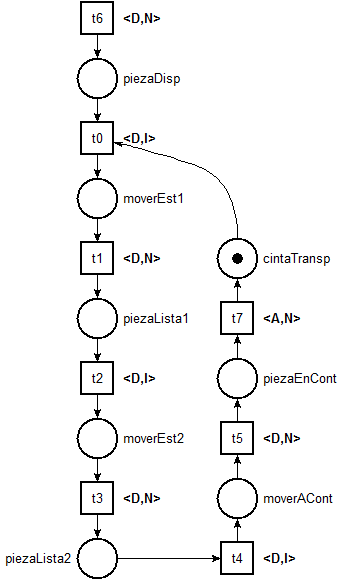
\includegraphics[height=100mm]{Petri_Cinta_Transportadora_2}
    \caption{Red de Petri de una cinta transportadora sincronizada por inserción
    de plaza-transición}
    \label{fig:petri_cinta_transportadora_2}
\end{figure}


A continuación se detalla la ejecución de la red de la
Figura~\ref{fig:petri_cinta_transportadora_2}:\\
\begin{enumerate}
	\item Se generan eventos que se encolan en la cola de entrada en
	``ejecutar\_accion\_1'', ``ejecutar\_accion\_2'', ``ejecutar\_mov\_cont''.
	\item El monitor bloquea los hilos que generaron eventos para
	``ejecutar\_accion\_1'', ``ejecutar\_accion\_2'', ``ejecutar\_mov\_cont''
	por no estar sensibilizadas las transiciones en ese momento.
	\item Llega una pieza y se genera un evento de entrada en “recibir\_pieza”
	\item El monitor dispara “recibir\_pieza” y se coloca un token en “piezaDisp”,
		sensibilizando “ejecutar\_accion\_1”.
	\item El monitor libera el hilo bloqueado en “ejecutar\_accion\_1” ya que ahora tiene permiso
		de ejecución.
	\item Se ejecuta la acción “accion\_1”. Una vez finalizado se genera un evento
	que se envía a la cola de entrada de “finalizar\_acc\_1”.
	\item Como “finalizar\_acc\_1” está sensibilizada el monitor la dispara y se coloca un token
		en “piezaLista1”, sensibilizando “ejecutar\_accion\_2”.
	\item El monitor libera el hilo bloqueado en “ejecutar\_accion\_2” ya que ahora
	tiene permiso de ejecución.
	\item Se ejecuta la acción “accion\_2”. Una vez finalizado se genera un evento
	que se envía a la cola de entrada de “finalizar\_acc\_2”.
	\item Como “finalizar\_acc\_2” está sensibilizada el monitor la dispara y se
	coloca un token en “piezaLista2”, sensibilizando “ejecutar\_mov\_cont”.
	\item El monitor libera el hilo bloqueado en “ejecutar\_mov\_cont” ya que ahora tiene permiso
		de ejecución.
	\item Se ejecuta la acción “movimiento\_a\_cont”. Una vez finalizado se genera
	un evento que se envía a la cola de entrada de “finalizar\_mov\_cont”
	\item Como “finalizar\_mov\_cont” está sensibilizada el monitor la dispara y se coloca un token
		en ``piezaEnCont''.
	\item Se dispara la transición ``liberar\_cinta'', que es automática, y se
	libera el recurso ``cintaTransp''.
\end{enumerate}

La principal ventaja de este método consiste en no modificar la semántica de
la red y no añadir nuevos conceptos ni cambios en la forma de ejecución.
La desventaja más importante es que provoca un incremento considerable de
la cantidad de plazas y transiciones de la red, lo que conlleva el
procesamiento de matrices de mayor tamaño. En la
sección~\ref{sec:complex_secuential_task_controller} se estudia un método que
permiten contrarrestar el aumento de tamaño de la RdP para procesos
secuenciales.

\subsubsection{Evento de Finalización de Acción por Guardas}
En la Figura~\ref{fig:petri_cinta_transportadora_3} se observa un modelo de
RdP para la sincronización de acciones mediante petición de ejecución, con aviso
de finalización de acción por guardas. Este método consiste en la utilización de
una guarda como forma de sincronización entre acciones consecutivas.

\begin{figure}[H]
    \centering
    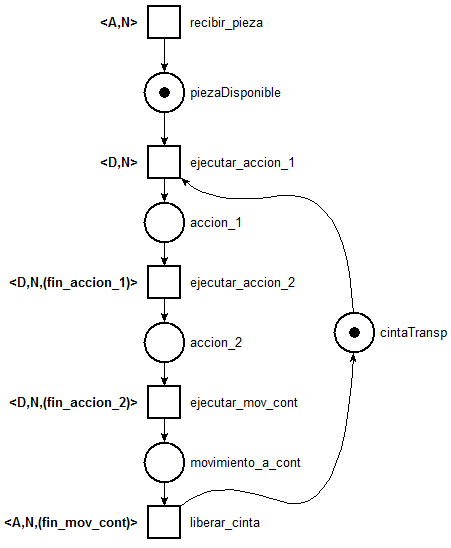
\includegraphics[height=100mm]{Petri_Cinta_Transportadora_3}
    \caption{Red de Petri de una cinta transportadora sincronizada por guardas.}
    \label{fig:petri_cinta_transportadora_3}
\end{figure}

A continuación se detalla la ejecución de la red de la
Figura~\ref{fig:petri_cinta_transportadora_3}
\begin{enumerate}
    \item Se generan eventos que se encolan en la cola de entrada en
    ``ejecutar\_accion\_1'', ``ejecutar\_accion\_2'', ``ejecutar\_mov\_cont''.
	\item El monitor bloquea los hilos que generaron eventos para
	``ejecutar\_accion\_2'' y ``ejecutar\_mov\_cont'' por no estar sensibilizadas
	las transiciones en ese momento.
	\item Se dispara ``ejecutar\_accion\_1'' y se coloca un token en ``accion\_1''.
	Comienza la ejecución de la acción ``accion\_1''. La transición
	``ejecutar\_accion\_2' no se encuentra sensibilizada dado que la guarda
	``fin\_accion\_1'' tiene estado ``false''.
	\item Finaliza la ejecución de ``accion\_1'' y se establece la guarda
	``fin\_accion\_1'' con estado ``true''.
	\item Al estar sensibilizada ``ejecutar\_accion\_2'', se dispara y se libera el hilo
	bloqueado en su cola de condición. Se coloca un token en ``accion\_2'' y
	comienza la ejecución de esta acción. La transición ``ejecutar\_mov\_cont'' no
	se encuentra sensibilizada dado que la guarda ``fin\_accion\_2'' tiene estado
	``false''.
	Se establece la guarda ``fin\_accion\_1'' a ``false'' nuevamente.
	\item Finaliza la ejecución de ``accion\_2'' y se establece la guarda
	``fin\_accion\_2'' con estado ``true''.
	\item Al estar sensibilizada ``ejecutar\_mov\_cont'', se dispara y se libera
	el hilo bloqueado en su cola de condición. Se coloca un token en
	``movimiento\_a\_cont'' y comienza la ejecución de esta acción. La transición
	``liberar\_cinta'' no se encuentra sensibilizada dado que la guarda
	``fin\_mov\_cont'' tiene estado ``false''.
	Se establece la guarda ``fin\_accion\_1'' a ``false'' nuevamente.
	\item Finaliza la ejecución de ``movimiento\_a\_cont'' y se establece la guarda
	``fin\_mov\_cont'' con estado ``true''.
	\item Al estar sensibilidada, se dispara la transición ``liberar\_cinta'', que es
	automática, y se libera el recurso ``cintaTransp''. Se establece la guarda
	``fin\_mov\_cont'' a ``false'' nuevamente.
\end{enumerate}

La ventaja de este método es que permite resolver el problema de sincronización
sin aumentar la cantidad de componentes de la red de Petri.
Como desventaja se puede mencionar que el diseño
del monitor de petri soporta una única guarda por transición, por lo tanto esta
solución impide la utilización de la guarda para otros propósitos. Otra
desventaja importante de la utilización de guardas es que al ser un valor
binario, lleva a una pérdida de eventos de finalización cuando
múltiples hilos realizan una misma acción.

Con el fin de ejemplificar la pérdida de eventos de finalización al utilizar
sincronización de finalización de acción por guardas se analiza el siguiente
caso de ejemplo:
\begin{labeling}{description}
\item [Ejemplo]
	Una ``tarea A'' es realizada por multiples hilos de manera independiente, y cada
	hilo realiza la ``tarea A'' en su totalidad. A su vez una ``tarea B'', que
	debe realizarse luego de la finalización de la ``tarea A'', es ejecutada por
	un único hilo. En este caso la utilización de guardas podría llevar a una
	pérdida de eventos de finalización de la ``tarea A'' debido a la condición
	binaria de la guarda. En la red de la Figura
	~\ref{fig:ejecucion_multiples_hilos_guardas}, un máximo de 5 hilos puede
	ejecutar la ``tarea A'' al mismo tiempo. En el estado que muestra la
	figura existen tres hilos corriendo la ``tarea A''. De acuerdo al planteo de
	este problema, la ``tarea B'' es ejecutada por un único hilo. Cuando dos o más
	hilos finalizan la ``tarea A'' y establecen la guarda ``Fin\_TareaA'' en ``true'',
	existe la posibilidad de que otro hilo dispare ``t1'' antes de comenzar la
	ejecución de la ``tareaB''. En este momento, el hilo que dispara ``t1''
	modifica el valor de la guarda ``Fin\_TareaA'' a ``false'', sobreescribiendo
	el aviso de finalización de acción de los hilos que ya habían establecido
	``Fin\_TareaA'' en ``true''. De esta manera, se pierden eventos de aviso de fin
	de ejecución, provocando la incorrecta sincronización del sistema.
\end{labeling}

\begin{figure}[H]
    \centering
    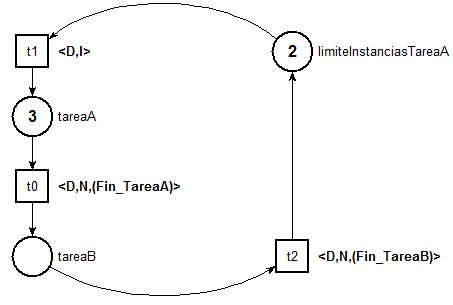
\includegraphics[height=60mm]{Ejecucion_Tarea_Multiples_Hilos_Guardas}
    \caption{RdP: Problema de sincronización de acciones dependientes usando
    guardas, debido a su condición binaria}
    \label{fig:ejecucion_multiples_hilos_guardas}
\end{figure}


\subsubsection{Evento de Finalización de Acción por Cola de Condición de
Disparo No Perenne}
En la Figura~\ref{fig:petri_cinta_transportadora_4} se observa un modelo de
RdP para la sincronización de acciones mediante petición de ejecución, con aviso
de finalización de acción por cola de condición de disparo no perenne. 
Esta forma de solucionar la sincronización de acciones dependientes
supone añadir una nueva propiedad ``P'' a las transiciones. Los hilos
bloqueados en la cola de condición de una transición con propiedad ``P'' sólo
se liberan cuando la transición se encuentra habilitada y además un hilo
externo realiza un disparo no perenne sobre la transición.

\begin{figure}[H]
    \centering
    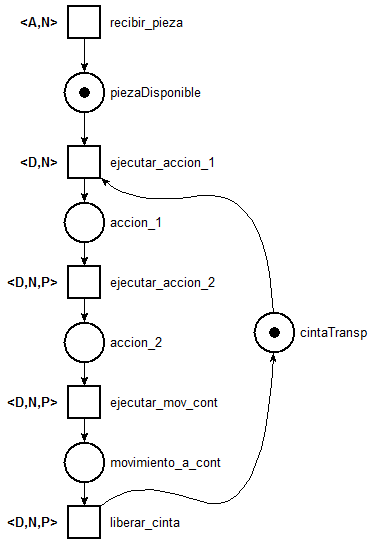
\includegraphics[height=100mm]{Petri_Cinta_Transportadora_4}
    \caption{Red de Petri de una cinta transportadora sincronizada por
    propiedad ``P''.}
    \label{fig:petri_cinta_transportadora_4}
\end{figure}

\begin{enumerate}
    \item Se generan eventos que se encolan en la cola de entrada en
    ``ejecutar\_accion\_1'', ``ejecutar\_accion\_2'', ``ejecutar\_mov\_cont'',
    y ``liberar\_cinta''.
	\item El monitor bloquea los hilos que generaron eventos para
	``ejecutar\_accion\_2'', ``ejecutar\_mov\_cont'', y ``liberar\_cinta'' por
	no estar sensibilizadas las transiciones en ese momento.
	\item Se dispara ``ejecutar\_accion\_1' y se coloca un token en ``moverEst1''.
	Comienza la ejecución de la acción ``accion\_1''. La transición
	``ejecutar\_accion\_2'' no se dispara ya que es de tipo ``P''.
	\item Finaliza la ejecución de ``accion\_1'' y un hilo dispara 
	``ejecutar\_accion\_2'' de forma no perenne para dar aviso de la finalización
	de la acción.
	\item Se libera el hilo bloqueado en cola de condición de
	``ejecutar\_accion\_2''. Se coloca un token en ``accion\_2'' y comienza la
	ejecución de esta acción. La transición ``ejecutar\_mov\_cont'' no se dispara
	ya que es de tipo ``P''.
	\item Finaliza la ejecución de ``accion\_2'' y un hilo dispara
	``ejecutar\_mov\_cont'' de forma no perenne para dar aviso de la finalización
	de la acción.
	\item  Se libera el hilo bloqueado en cola de condición de
	``ejecutar\_mov\_cont''. Se coloca un token en ``movimiento\_a\_cont'' y
	comienza la ejecución de esta acción. La transición ``liberar\_cinta'' no se dispara ya
	que es de tipo ``P''.
	\item Finaliza la ejecución de ``movimiento\_a\_cont'' y un hilo dispara
	``liberar\_cinta'' de forma no perenne para dar aviso de la finalización de la
	acción.
	\item Se libera el recurso ``cintaTransp''.
\end{enumerate}

La ventaja de esta solución es que no incrementa el numero de componentes de la
red. Su principal desventaja consiste en que añade una nueva etiqueta a la
RdP, dificultando su validación matemática. Esta solución supone añadir
una interfaz al monitor de Petri para bloquear hilos en una cola de condición de
una transición tipo P y que los hilos bloqueados en esta cola de condición sólo
puedan liberarse por medio de un disparo no perenne ocasionado por un hilo
externo.
El hilo que realiza el disparo sobre la transición debe realizar una operación
\emph{release} sobre la cola de condición de disparos no perennes (sin importar
si existen o no hilos bloqueados en la cola) para evitar la pérdida de eventos de
finalización de acción.

\subsection{Resumen de Modos de Sincronización}
\label{sec:resumen_sincronizacion}
Existen dos maneras de coordinar la ejecución de las acciones a partir de una
red de Petri.\\ 
\begin{enumerate}
  \item \textbf{Sincronización por aviso de ejecución: } Consiste en suscribir
  una acción a una transición, que envía una notificación en el momento en que
  es disparada. Ante un informe de esta transición, la acción suscripta
  comienza su ejecución.
  Al finalizar una acción, se dispara la transición a la cual está suscripta la
  siguiente acción a ejecutar.
  La principal desventaja de este método consiste en la descentralización del
  manejo de los hilos por parte del monitor, lo cual va en contra de los objetivos del
  proyecto.
  \item \textbf{Sincronización por petición de ejecución: } Los hilos que
  ejecutan acciones realizan una peticion de ejecución al monitor (mediante el
  disparo de transiciones), sin tener en cuenta el estado actual de la red de
  Petri. De este modo el monitor bloquea los hilos que no pueden ejecutarse y
  libera los hilos que cumplan con las condiciones de ejecución. El manejo de
  la concurrencia es llevado a cabo íntegramente por el monitor.
  Para sincronizar acciones dependientes entre sí (una debe comenzar luego de
  la finalización de la otra) se requiere un modo de dar aviso al monitor de
  la finalización de una acción. Se analizan tres opciones:
  \begin{itemize}
      \item Evento de finalización de acción por grupo transición-plaza
	  \item Evento de finalización de acción por guardas
	  \item Evento de finalización de acción por cola de condición de disparo no
	  perenne.
  \end{itemize}
  Se optó por adoptar el evento de finalización de acción por grupo
  transición-plaza. Esta forma presenta la ventaja de no añadir
  conceptos nuevos a la RdP, facilitando el entendimiento de la misma. Además
  no presenta pérdida de eventos de finalización de acción.
  La principal desventaja del grupo transición-plaza consiste en el incremento
  del tamaño de la RdP. En procesos secuenciales, puede contrarrestarse mediante
  el uso del controlador de acciones descripto en la
  sección~\ref{sec:complex_secuential_task_controller}.
\end{enumerate}
 

 
 
 
 
